\documentclass[12pt]{article}
\usepackage{etex}
\usepackage{etex}
\usepackage{enumitem}
\usepackage[round]{natbib}
\bibliographystyle{plainnat}

%Below are necessary packages for your course.
\usepackage{amsfonts,latexsym,amsthm,amssymb,amsmath,euscript}
\usepackage{mathrsfs,manfnt,enumitem,stmaryrd}
% \usepackage[super]{nth}
\usepackage{setspace}
\usepackage{titlesec}
\usepackage{framed}
\usepackage{verbatim}
\usepackage{xcolor}
\usepackage{calc,color,relsize}
\usepackage{amsxtra}
\usepackage[utf8]{inputenc}
%\usepackage{eucal}
% \usepackage[all]{xy}
\usepackage{graphicx}
\usepackage[geometry]{ifsym}
\usepackage{hyperref}
    \hypersetup{colorlinks=true,citecolor=blue,urlcolor=black,linkbordercolor={1 0 0}}
\usepackage{cleveref}
\usepackage{mathtools}
%\usepackage{fc}
\usepackage{pifont}
\usepackage{tikz}
\usepackage{tikz-cd}
\usetikzlibrary{matrix,arrows,decorations.pathmorphing}

\setlength\topmargin{0pt}
\addtolength\topmargin{-\headheight}
\addtolength\topmargin{-\headsep}
\setlength\oddsidemargin{0pt}
\setlength\textwidth{\paperwidth}
\addtolength\textwidth{-2in}
\setlength\textheight{\paperheight}
\addtolength\textheight{-2in}
\usepackage{layout}

\allowdisplaybreaks[1]


%Below are the theorem, definition, example, lemma, etc. body types.

\newtheorem{theorem}{Theorem}
\newtheorem*{proposition}{Proposition}
\newtheorem{lemma}[theorem]{Lemma}
\newtheorem{corollary}[theorem]{Corollary}
\newtheorem{conjecture}[theorem]{Conjecture}
\newtheorem{postulate}[theorem]{Postulate}
\theoremstyle{definition}
\newtheorem{defn}[theorem]{Definition}
\newtheorem{example}[theorem]{Example}

\theoremstyle{remark}
\newtheorem*{remark}{Remark}
\newtheorem*{notation}{Notation}
\newtheorem*{note}{Note}

% \DeclareUnicodeCharacter{1F346}{\eggplant}

%This is a list of new commands I defined to make your life easier. Use them as the occur in the course.
\newcommand{\sub}{\operatorname{sub}}
\newcommand{\quot}{\operatorname{quot}}
\newcommand{\bw}{\bigwedge}
\newcommand{\Avs}{\operatorname{Av}^{\operatorname{sign}}}
\newcommand{\bad}{\operatorname{bad}}
\newcommand{\sign}{\operatorname{sign}}
\newcommand{\id}{\operatorname{id}}
\newcommand{\defeq}{\vcentcolon=}
\newcommand{\eqdef}{=\vcentcolon}
%We can even define a new command for \newcommand!
\newcommand{\nc}{\newcommand}
\nc{\on}{\operatorname}
\nc\renc{\renewcommand}
\nc{\BR}{\mathbb R}
\nc{\BG}{\mathbb G}
\nc{\BP}{\mathbb P}
\nc{\BC}{\mathbb C}
\nc{\BQ}{\mathbb Q}
\nc{\BF}{\mathbb F}
\nc{\BZ}{\mathbb Z}
\nc{\BN}{\mathbb N}
\nc{\BS}{\mathbb S}
\nc{\Hom}{\on{Hom}}
\nc{\wt}{\widetilde}
\nc{\vspan}{\on{span}}
\nc{\ord}{\on{ord}}
\nc{\im}{\on{im}}
\nc{\Mat}{\on{Mat}}
\nc{\can}{\on{can}}
\nc{\coker}{\on{coker}}
\nc{\ev}{\on{ev}}
\nc{\Tr}{\on{Tr}}
\nc{\End}{\on{End}}
\nc{\swap}{\on{swap}}
\nc{\Set}{\on{Set}}
\nc{\bC}{{\mathbf C}}
\nc{\bc}{{\mathbf c}}
\nc{\bD}{{\mathbf D}}
\nc{\bd}{{\mathbf d}}
\nc{\bE}{{\mathbf E}}
\nc{\be}{{\mathbf e}}
\nc{\bF}{{\mathbf F}}
\nc{\bff}{{\mathbf f}}
\nc{\CE}{\mathcal E}
\nc{\CD}{\mathcal D}
\nc{\CH}{\mathcal H}
\nc{\CY}{\mathcal Y}
\nc{\CN}{\mathcal N}
\renc{\mod}{\on{-mod}} %Careful - turn this off in a number theory setting
\newcommand{\spec}{\text{spec}}
\nc{\adj}{\on{adj}}
\nc{\tensor}[3]{#1 \underset{#2}\otimes #3}
\nc{\Nat}{\on{Nat}}
\nc{\op}{\on{op}}
\nc{\Funct}{\on{Funct}}
\nc{\Ob}{\on{Ob}}
\nc{\fR}{\mathfrak{R}}
\nc{\Vect}{\on{Vect}}
\nc{\ns}{\on{non-spec}}
\nc{\ol}{\overline}
\nc{\ul}{\underline}
\nc{\univ}{\on{univ}}
\nc{\Maps}{\on{Maps}}
\nc{\bdd}{\on{bdd}}
\nc{\cont}{\on{cont}}
\nc{\Sym}{\on{Sym}}
\nc{\vol}{\on{vol}}
\nc{\supp}{\on{supp}}
\nc{\Lie}{\on{Lie}}
\nc{\master}{\on{master}}
\nc{\pt}{\on{pt}}

\nc{\dx}{\on{dx}}
\nc{\dy}{\on{dy}}
\nc{\dtheta}{\on{d}\theta}
\nc{\hleft}{h_{\shortrightarrow}}
\nc{\hleftt}{h_{\shortrightarrow, t}}
\nc{\hright}{h_{\shortleftarrow}}
\nc{\hrightt}{h_{\shortleftarrow, t}}

\renewcommand{\v}[1]{\mathbf{#1}}

% custom rachit code
% \everymath{\displaystyle}
\newcommand{\Var}{\on{Var}}
\newcommand{\E}{\mathbb{E}}
\newcommand{\Bern}{\on{Bern}}
\newcommand{\Beta}{\on{Beta}}
\newcommand{\Kumar}{\on{Kumaraswamy}}
\newcommand{\Expo}{\on{Expo}}
\newcommand{\Prob}{\mathbb{P}}
\newcommand{\Like}{{\mathcal L}}
\newcommand{\norm}[1]{\left\lVert#1\right\rVert}
\newcommand{\inprod}[1]{\left\langle#1\right\rangle}
\definecolor{textgrey}{HTML}{BBBBBB}
\newenvironment{problem}{\par\color{blue}}{\par}
\DeclarePairedDelimiter\ceil{\lceil}{\rceil}
\DeclarePairedDelimiter\floor{\lfloor}{\rfloor}
\DeclarePairedDelimiter\abs{\lvert}{\rvert}%

\DeclarePairedDelimiterX{\infdivx}[2]{(}{)}{%
  #1\;\delimsize\|\;#2%
}
\newcommand{\kldiv}{KL\infdivx}

\usepackage{ifthen,xcolor}
\newlength{\tabcont}

\title{\large Particle-filter based language models\vspace{-0.5in}} % Change the PSet number as needed.

\begin{document}

\maketitle

\vspace*{-0.25in}
\centerline{Rachit Singh, Yuntian Deng}
\centerline{\href{mailto:rachitsingh@college.harvard.edu}{{\tt rachitsingh@college.harvard.edu}}}
\vspace*{0.15in}
\medskip

We were discussing methods for inducing multimodality into tasks like translation or summarization. A lot of approaches are looking at forming a distribution over latent vectors that encode the entire sentence together, but we decided to look at the problem from the perspective of localized changes. So, instead of taking a variational distribution $q(z)$ over the hidden state before passing through a decoder, we thought it might be interesting to instead draw at each time step from a distribution $z_t \sim q_t(z_t; \lambda_t)$ and form the generated word from the distribution $p(y_t | z, y_{1:t-1})$. 

\smallskip

This has the downside of not leading directly to a "sentence representation", since the sequence of encoded vectors is as long as the sentence itself, but our guess is that generation is more natural, if we can find the right representation $q$. For example, if we initialize the prior distribution of $\v z$ to be the empirical distribution of part-of-speech tag sequences we find in the training data, then we might softly contrain the model $\v q$ to be close to these sequences.

\subsection*{Generative Model}

To formalize the idea, we have the following generative process:
\begin{align}
	\v z &\sim p(\v z) = \prod_{t = 1}^m p(z_t \mid \v z_{1:t-1}) \\
	\v y &\sim p(\v y | \v z) = \prod_{t = 1}^m p(y_t \mid \v y_{1:t-1}, z_t) \\
	z_t &\sim p(z_t | \v z_{1:t-1}) = \on{Cat}(\lambda^z_t) \\ 
	y_t &\sim p(y_t | z_{t}, \v y_{1:t-1}) = \on{Cat}(\lambda^y_t)
\end{align}
Where the parameters $\lambda^z_t, \lambda^y_t$ are computed using recurrent neural networks. Assuming that $\v \hleft, \v \hright$ are the hidden states corresponding to the traversal of a bidirectional RNN over $\v y$, we can compute a sequence of hidden states $h^e_t, h^d_t$: 
\begin{align*}
	h^e_t &= \on{RNN}(h^e_{t - 1}, \hleftt, \hrightt, z_{t - 1}) \\
	\lambda^z_t &= f(h^e_t) \\
	h^d_t &= \on{RNN}(h^d_{t - 1}, \hleftt, \hrightt, y_{t - 1}) \\
	\lambda^y_t &= g(h^d_t)
\end{align*}
where RNN corresponds to any RNN structure (e.g. a GRU or LSTM), and $f, g$ might correspond to a linear map into the output space. The BiRNN could be replaced with a regular RNN to reduce complexity. This is not equivalent to a state space model as considered by \citep{krishnan2017structured}, since for that model the transition distribution for $z_t$ only depends on the previous $z_{t-1}$, and the emission distribution for $y_t$ only depends on the latent variable $z_t$. We think that such a simple model doesn't capture the dependencies of natural language.

\subsection*{Inference}

We can use several different variational approximations that might lead to more powerful approximation. The straightforward approach is to use 
$$q(\v z | y) = q(z_1 | y)\prod_{i = 2}^{L} q(z_i | z_{i - 1}, y)$$
One potential change is that we can factor the variational distribution using what is called a 'top-down variational approximation': we can allow 
$$q(\v z | y) = q(z_L | y)\prod_{i = 1}^{L - 1} q(z_i | z_{i + 1}, y)$$
(note that the posterior is factored in reverse). \citet{sonderby2016ladder} uses this technique in \emph{ladder variational autoencoders} (LVAE). \citet{krishnan2017structured} also indicates that doing inference in reverse might make more sense.

While we have a somewhat clearer sense of what the generative model should look like, we have a lot of choice over \emph{what} our hidden variables are. For example, we can assume that they they're Gaussian, or possible a discrete random variable. 

\medskip

We also have significant choice over the prior in these case. Since we want the prior to be over the entire vector $\v z$, we can factor the prior over time as well. 

\subsection*{Particle Filter}

Recent work (\citet{naesseth2017variational, maddison2017filtering}) has shown how to find a significantly tigher variational bound in the case of sequential latent distributions (see \cref{fig:vsmc}). Essentially, by treating the sequence of samples (i.e. collection of samples for $z_1$, another as $z_2$, etc.) as the progressive states of a particle filter, we can do better than the naive approach of sampling $k$ separate chains, by using a \textit{resample/reweight} step to remove low weight sequences and resample high weight sequences. In effect, this is a form of probabilistic, differentiable beam search - we can essentially optimize the proposal distribution $p(z_t | \v z_{1:t-1}, \v y)$, but only if the corresponding predictions are good. 

\smallskip

There's also some room for exploration here, since both implementations above appear to use black-box variational inference for the \textit{resample/reweight} step, since the choice of which particles to use as an ancestor is discrete, and it's not acceptable to have 'points in the simplex' as in the Concrete distribution. However, the paper we recently read in reading group (Backpropagation through the Void) might prove better suited for this task, which is something to explore given time.

\subsubsection*{Disadvantages}
One primary disadvantage is that the addition of another sequential model (i.e. a decoder) for predicting the latent state distribution increases the number of parameters significantly. Our approach for dealing with this concern is to reduce the size of the latent representation $\v z$. Since we're stretching the latent representation over the entire sequence, we can let $z_t \in [k]$ rather than $z_t \in \BR^{k}$, and reduce the amount of inference necessary. In general using a discrete latent space is difficult for inference, but recent advancements have made this problem less difficult. Still, since we can only sample a very small subset of the possible sequences (and they are totally disjoint), we might have trouble early in the training process.  

\subsubsection*{Advantages} 
\begin{enumerate}
	\item \textbf{A tighter approximation to the marginal might lead to multimodality in our responses}: The reason is this: suppose that we're in the autoencoder setting, and we have derived parameters $\lambda = f(\v x)$ for the variational distribution $q(\v z; \lambda)$. If we take multiple samples $\v z_1, \v z_2, \ldots \v z_k$, and calculate the log-joint $\log p(\v x, \v z_i)$ for each of them, we'll get several values. If we're properly multimodal, then one of the $\v z_i$ might correspond to a exact phrasing of $\v x$ that we have (rather than a rearrangement or rephrasing) and so $\log p(\v x, \v z_i)$ might be high, while all of the other log-joints are very small. Then, taking the log-sum-exp of these values (corresponding to $\log \sum_{i}^k p(\v x, \v z_i)$) will still be high, even though most of the other predictions are bad, which is what we want. So our usual metric of the ELBO would score this poorly, even though this metric (the IWAE bound) would score it high. In particular, as $k \to \infty$, the evaluation gets closer to what we want, and also the bound goes to the true marginal $\log p(x)$. 
	\item \textbf{It might be more interpretable}: in general, it's difficult to interpret the latent space learned by a single vector $\v z$. Even though the latent sequence $[z_1, z_2, \ldots, z_m]$ is not more likely to be interpretable, it's possible that we can force it to be so. For example, we might constrain training on this portion of the model early by letting $\v z$ be exactly the POS tags for the sequence $\v y$, and then train the inference network later once we have 'locked in' what the indicator $z_t$ mean. Alternatively, we can restrict the generative model $p(y_t \mid z_t \ldots)$ to only generate words that correspond to the POS tag $z_t$ (again, from the true $\v y$) to bootstrap training. Another idea is to constrain $p(\v z \mid \v x)$ to be limited to sequences that we've seen in the training data. This also tackles the perpetual issue of identifiability of neural models. 
\end{enumerate}

\begin{figure}[t]
  % \vspace{-5mm}
  \begin{center}
    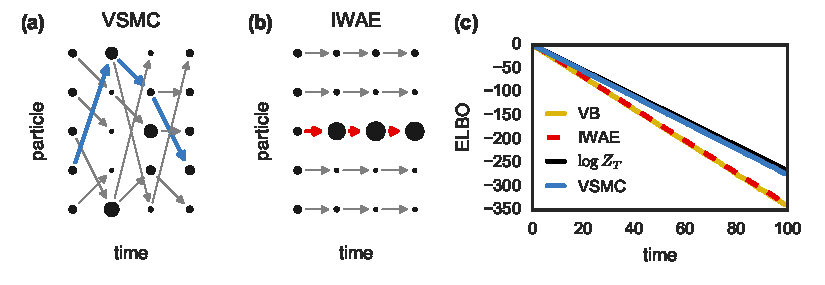
\includegraphics{vsmc.pdf}
  \end{center}
  \vspace{-5mm}
  \caption{Comparing {VSMC} and the {IWAE} (from \citep{naesseth2017variational})
    (a) {VSMC} resamples the particles at each step, and chooses the most likely sequence, akin to beam search.
    (b) {IWAE} does the same, but without resampling, and only chooses one of the $k$ chains. This means that only one sequence might be sampled in general.
    (c) As time increases, IWAE and regular variational Bayes (VB) diverge from the true marginal likelihood, while VSMC stays close.}
  \label{fig:vsmc}
%\vspace{-5mm}
\end{figure}

\subsection*{Related work}
\textit{Unfortunately this section is a little less fleshed out than it should be}. Much of the work on using variational RNNs focuses on state space models \citep{krishnan2017structured,chung2015recurrent,naesseth2017variational,maddison2017filtering}. The main analogue of this work is the neural variational translation model of \citet{zhang2016variational}), which uses a single latent state for translation, and \citet{li2017deep}, which also uses sequential latent variables for the task of summarization, but which use Gaussian latent variables and don't tackle the identifiability concern as above, and don't use the particle-filter bound to tighten the objective. 

\smallskip

[side note: \citet{li2017deep} say they are beating state of the art on summarization, but isn't the pointer-generator networks SOTA right now? they don't compare]  

\subsection*{Plan of attack}
Let me know if this makes sense (my intuition is not great):

\begin{enumerate}
\item Build an autoencoder that uses the above generative model and inference network, and train it to work without a tighter bound on PTB [1-2 weeks]
\item Add attention if that makes sense [1 week?]
\item Add the particle filter bound, and measure the improvement [2 weeks]
\item Spend a lot of time trying variants [winter break]
\end{enumerate}

\bibliography{proposal}

\end{document}	